\documentclass[11pt,a4paper,titlepage,oneside]{report}
\usepackage{titling}
\usepackage{graphicx}
\usepackage{mathtools}
\usepackage{lmodern}
\usepackage{amsmath}
\usepackage{float}

%% Memoir layout setup

%% NOTE: You are strongly advised not to change any of them unless you
%% know what you are doing.  These settings strongly interact in the
%% final look of the document.

% Dependencies
\usepackage{bfhlogo}
\usepackage{etoolbox}% http://ctan.org/pkg/etoolbox

\makeatletter
%%begin novalidate
%% Titlepage adjustments
\pretitle{\vspace{0pt plus 0.7fill}\begin{center}\Huge}
\posttitle{\end{center}\par}
\preauthor{\par\begin{center}\let\and\\\Large}
\postauthor{\end{center}}
\predate{\par\begin{center}\Large}
\postdate{\end{center}}
%%end novalidate
\def\@advisors{}
\newcommand{\advisors}[1]{\def\@advisors{#1}}
\def\@department{}
\newcommand{\department}[1]{\def\@department{#1}}
\def\@thesistype{}
\newcommand{\thesistype}[1]{\def\@thesistype{#1}}

\renewcommand{\maketitlehooka}{\noindent\bfhlogo[2cm]}

\renewcommand{\maketitlehookb}{\vspace{1in}%
  \par\begin{center}\Large\sffamily\@thesistype\end{center}}

\renewcommand{\maketitlehookd}{%
  \vfill\par
  \begin{flushright}
    \sffamily
    \@advisors\par
    \@department, BFH
  \end{flushright}
}

% Fix the chapters (unnecessary space)
\patchcmd{\@makechapterhead}{\vspace*{50\p@}}{}{}{}% Removes space above \chapter head
\patchcmd{\@makeschapterhead}{\vspace*{50\p@}}{}{}{}% Removes space above \chapter* head

\makeatother

\setlength{\droptitle}{-48pt}


\title{Point cloud-based camera calibration}
\author{Stefan Eichenberger}
\date{August 2018}
\advisors{Marcus Hudritsch}
\department{TSM CPVR Lab}

\begin{document}
\maketitle

\begin{abstract}
To reconstruct the pose and position of a camera the intrinsic camera model must once be calculated. We show a method on how to calibrate a camera based on a pregenerated point cloud. This method makes camera calibration more user friendly for augmented reality applications where pregenerated point clouds can be used.
\end{abstract}

\tableofcontents

\chapter{Introduction}
In 1865 the Christoffeltower in Bern was destroyed to create space for the new railway station. In a today's point of view this decision was a mistake. They destroyed a part of Bern history back then.\\
Today the area around the railway station is heavily used by buses and cars. Therefore, it is impossible to reconstruct the tower physically. Luckily we nowadays have the technology to at least create the illusion of such a building. The idea is to create a virtual Chritoffeltower by using augmented reality.\\
One problem of this idea is that we don't know what kind of device a possible viewer will have. Therefore it is not possible to use calibration data of a predefined type. It must be possible to calibrate the camera right in place. This is where this project comes in.\\
The goal of this project is to calibrate a camera based on a pregenerated point cloud. The point cloud must be generated anyhow for this project to allow estimating the position of the viewer. This point cloud can also be used to calibrate the camera. 

\section{Goals}
A program should be written that takes as input a 3d point cloud and 2d points and calculates the camera model from these points. The whole project consists of the following parts:
\begin{itemize}
\item Search for existing solution
\item Get used to the topic SLAM, AR and 3D representation
\item Choose a programming environment (Python, Matlab)
\item Implemnet a proof of concept with syntetic data
\item Implement a proof of concept with real data
\end{itemize}

\chapter{Evaluation}

As a first task papers about existing methods are studied. This includes similar approaches which are not 100\% the same.

\section{Existing methods}
\subsection{Checkerboard}\label{sec:checkerboard}
The most famous variant for camera calibration is the checkerboard approach \cite{zhang}. For this approach one must take photos of a checkerboard. The algorithm then performs the following tasks:
\begin{enumerate}
  \item Search the checkerboard corners
  \item Find an approximation of the extrinsic matrix
  \item Find an approximation of the intrinsic matrix
  \item Solve the non linear camera model by minimizing the reprojection error with levenberg-marquart
\end{enumerate}

\subsection{Self-calibration with planar scene}
In comparison to the checkerboard calibration this approach doesn't need a checkerboard. It uses the same technique as checkerboard calibration but instead of using a known image any planar image can be used for calibration \cite{selfcalib}. The algorithm tries to estimate the camera model by doing a bundle adjustment over several images. In comparison to the checkerboard calibration this is more computational expensive and requires more images for doing the calibration.

\subsection{Decision}
Because the Checkerboard calibration is widely used and well documented, this method has been chosen for this project. We don't have a checkerboard available but a 3d cloud instead, so we have more information available as the Self-calibration approach needs. However, as we will see in chapter \ref{chap:implementation} this method needs some modification to the checkerboard calibration to fulfill our requirements.

\section{Tools}
\subsection{Matlab}
Matlab does have a powerful imaging toolbox. Besides that Matlab also has a lot of powerful tools to plot images, graphs etc. Matlab is a proprietary product of Mathworks.

\subsection{Python}
For experimenting and implemnting the proof of concept, Python has been chosen as the prefered programmming language. The reason for Python is that it has extremely good frameworks for doing scintific tasks and OpenCV has out of the box support for Python. So the additional Python frameworks are:
\begin{itemize}
  \item Scipy
    \subitem Adds some missing mathematically functions like Levenberg-Marquardt or linear least squares
  \item Numpy
    \subitem Is a verry powerful framework for handling matrixes
  \item OpenCV
    \subitem Adds all the necessary image processing features
  \item VisVis
    \subitem Allows GPU accelerated visualisation in Python
\end{itemize}

\subsection{Decision}
Because Python has a fast growing community and because we can use OpenCV from within it, the decision was made to use Python as programing language. It should be easy to port code written in Python/OpenCV to CPP/OpenCV if required.

\chapter{Implementation}\label{chap:implementation}
\section{Optimization}
What we will later see is that to fit a camera model, we need an opitmization algorithm. We will use two different kind of optimization algorithms one is linear least squares which is an optimization algorithm that minimises lineare mean squares problems. A second algorithm we will use is the Levenberg-Marquardt algorithm which is used to solves nonlinear least squares. We will see later which algorithm we use for which problem.

\subsection{Linear least squares}
Assume you have a problem in the form show in equation \ref{eq:least_squares_example1}.
\begin{equation}\label{eq:least_squares_example1}
  A*X=B \\ 
  \begin{pmatrix}
    a_{11} a_{12} \\
    a_{21} a_{22}
  \end{pmatrix}*
  \begin{pmatrix}
    x_1 \\
    x_2
  \end{pmatrix}=
  \begin{pmatrix}
    b_1 \\
    b_2
  \end{pmatrix}
\end{equation}
Where:
\begin{align*}
  a		  &: \text{known input values}\\
  x	  	&: \text{unkonwns}\\
  b		  &: \text{known output values}
\end{align*}
We try to find x. This is easy doable by inverting Matrix A and multiply the inverse with B. This will give us the unknown matrix X. We assume here that the matrix is non singular. Let us now assume we have more equations than unknowns which is a common use case in reality. We will then have something like in \ref{eq:least_squares_example2}. This example isn't solvable by inverting matrix A. Instead we need a new algorithm called linear least squares \ref{eq:least_squares_algorithm}. For more details on why this algorithm works see \cite{Monson}. Libraries that implement this kind of algorithms are often able to do a pseudo inverse instead of a simple inverse in case that a matrix is non singular. Such an implementation is e.g. pinv of numpy \cite{pinv}.
\begin{equation}\label{eq:least_squares_example2}
  A*X=B \\ 
  \begin{pmatrix}
    a_{11} a_{12} \\
    a_{21} a_{22} \\
    a_{31} a_{32} \\
    a_{41} a_{42}
  \end{pmatrix}*
  \begin{pmatrix}
    x_1 \\
    x_2
  \end{pmatrix}=
  \begin{pmatrix}
    b_1 \\
    b_2 \\
    b_3 \\
    b_4
  \end{pmatrix}
\end{equation}

\begin{equation}\label{eq:least_squares_algorithm}
  X=(A^H*A)^{-1}*A^H*B 
\end{equation}

An advantage of using a linear solver for the least squares problem is that it will always find the global minimum. It is also computaionally faster for problems with low to medium amount of unkowns (1-1000). However as the name states it can only solve problems where the unknowns are linear.

\subsection{Gradient-Descent}
Non-linear problems are much harder to solve. They can't guarantee to find the global optimum if the problems are non-convex. Probably one of the most common non-linear solvers is gradient descent. Gradient descent is an iterative algorithm which calculates the gradient at point x and then takes a step in the opposite direction of the gradient for minimizing a problem (see Figure \ref{fig:gradient_descent}). The update formula for gradient descent is shown in equation \ref{eq:gradient_descent}.
\begin{figure}[H]
  \begin{center}
    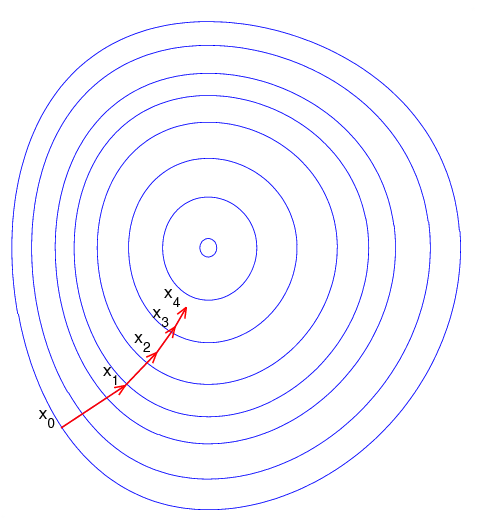
\includegraphics[width=0.5\textwidth]{img/gradient_descent.png}
  \end{center}
    \caption{Gradient descent}\label{fig:gradient_descent}
\end{figure}

\begin{equation}\label{eq:gradient_descent}
  x_{n+1}=x_n-\theta*\Delta f(x_n)
\end{equation}
Where:
\begin{align*}
  x		      &: \text{Parameters}\\
  \Delta f  &: \text{Derivation of function f to optimize}\\
  \theta    &: \text{Step size}
\end{align*}

\subsection{Newton}
The Gauss-Newton optimization algorithm is an algorithm that assumes a problem is approximately quadratic near the optimal solution. It does also derivate the function at a specific location but it will then jump immediately to the position where the derivation is zero (Figure \ref{fig:newton}). If the problem is quadratic near the optimal solution this algorithm converges faster than gradient descent. In comparison to the Newton algorithm, Gauss-Newton only works to minimize a sum of squared values. In comparison Newton works on all problems. However, Gauss-Newton has the advantage of being computational faster \cite{gauss_newton} because it doesn't need to compute the Hessian matrix. The update formula to solve for Gauss-Newton is shown in equation \ref{eq:gauss_newton}.

\begin{figure}[H]
  \begin{center}
    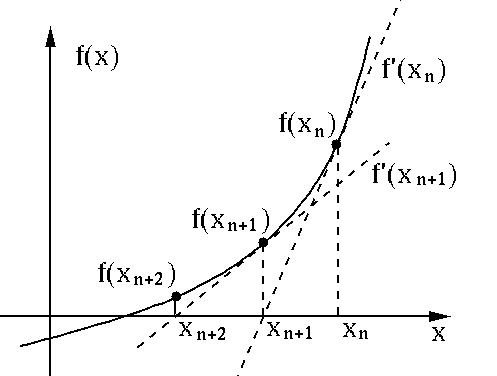
\includegraphics[width=0.5\textwidth]{img/newton.png}
  \end{center}
  \caption{Newton algorithm see \cite{newton_image}}\label{fig:newton}
\end{figure}

\begin{equation}\label{eq:gauss_newton}
  x_{n+1} = x_n - (J_n^T*J_n)^{-1}*J_n*e_n
\end{equation}
Where:
\begin{align*}
  x		  &: \text{Parameters to tune}\\
  n		  &: \text{Step}\\
  J		  &: \text{Jacobian}\\
  e  	  &: \text{The error y-ŷ}
\end{align*}


\subsection{Levenberg-Marquardt}
For this project Levenberg-Marquardt was chosen as non-linear optimization algorithm. This has been proposed by Zhang who first described the checkerboard calibration \cite{Zhang}. Levenberg-Marquardt uses Gauss-Newton which makes it fast to converge but can move to gradient descent if Gauss-Newton isn't converging. This makes this algorithm more robust than only using Gauss-Newton but makes it faster than gradient descent. Equation \ref{eq:levenberg_marquardt} shows the update equation for the parameters. \mu\ is the tuning parameter which will increase the influence of gradient descent. If \mu\ is very small (close to 0) then only Gauss-Newton is used. If \mu is huge then only gradient descent is used for optimization. \mu\ can be updated during optimization. If for example the error increases from step to step, then the influence of gradient descent must be increased because Gauss-Newton will never find an optimal solution.

\begin{equation}\label{eq:levenberg_marquardt}
  x_{n+1} = x_n - (J_n^T*J_n + \mu*I)^{-1}*J_n*e_n
\end{equation}
Where:
\begin{align*}
  x		  &: \text{Parameters to tune}\\
  n		  &: \text{Step}\\
  J		  &: \text{Jacobian}\\
  \mu	  &: \text{Learning coefficient for gradient descent}\\
  I     &: \text{Identity matrix}\\
  e  	  &: \text{The error y-ŷ}
\end{align*}

\section{Camera model}
The projection of an object in the 3 dimensional space onto a two dimensional image can be formulated as shown in equation \ref{eq:cm}.
\begin{equation}\label{eq:cm}
  \begin{pmatrix}fx & \gamma & cx \\
      0 & fy & cy \\
      0 & 0 & 1 \\
    \end{pmatrix}*
    \begin{pmatrix}
      r_{00} & r_{01} & r_{02} & tx \\
      r_{10} & r_{11} & r_{12} & ty \\
      r_{20} & r_{21} & r_{22} & tz \\
    \end{pmatrix}
    \begin{pmatrix}
      X \\
      Y \\
      Z \\
      1
    \end{pmatrix}=
    \begin{pmatrix}
      u \\
      v \\
      s
  \end{pmatrix}
\end{equation}
Where:
\begin{align*}
  X,Y,Z		&: \text{point in the 3d world}\\
  u,v	    	&: \text{point in a 2d image}\\
  s		&: \text{scaling factor (1 when normalized)}\\
  fx,fy   	&: \text{focal length of the camera}\\
  cx,cy   	&: \text{sensor displacement}\\
  tx,ty,tz	&: \text{translation with respect to the camera}\\
  r_{ij}	&: \text{part of the rotation matrix}
\end{align*}

We can explain this as following. A Point (X,Y,Z) is projected onto an image sensor (u,v) by the multiplication of an intrinsic times an extrinsic matrix. The extrinsic matrix describes how a point is rotated and translated with regards to the camera while the intrinsic matrix describes how the camera itself is constructed. For example in figure \ref{fig:projection} a point pi is rotated and translated to the objective of the camera. The point is then further transformed by the intrinsic camera matrix onto the image sensor.

\begin{figure}[H]
  \begin{center}
    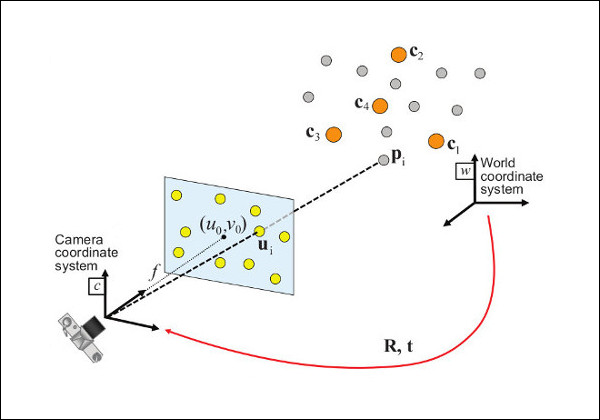
\includegraphics[width=0.5\textwidth]{img/pnp.jpg}
  \end{center}
    \caption{Point in 3D-space to image point}\label{fig:projection}
\end{figure}

When calibrating a camera we are interested in the intrinsic matrix because it will be constant over time for a specific camera. Additional to the intrinsic matrix a real world objective will have distortion. This means an image is not mapped perfectly onto the image plane but it is non linear distorted the further a pixel is placed from the principal point (cx,cy). How distortion affects the image is shown in equation \ref{eq:dist}.

\begin{equation}\label{eq:dist}
	\begin{pmatrix}\gamma_{u} \\
	  \gamma_{v}
	\end{pmatrix}=\begin{pmatrix}
	  u(k_1r^2+k_2r^4+k_3r^6)\\
	  v(k_1r^2+k_2r^4+k_3r^6)
	\end{pmatrix}+\begin{pmatrix}
	  2p_1uv+p_2(r^2+2u^2)\\
	  p_1(r^2+2v^2)+2p_2uv
	\end{pmatrix}
\end{equation}
\begin{equation}\label{eq:pdist}
\begin{pmatrix}u'\\v'\end{pmatrix}=\begin{pmatrix}
u\\v\end{pmatrix}+\begin{pmatrix}\gamma_{u}\\\gamma_{v}\end{pmatrix}
\end{equation}
Where:
\begin{align*}
  k_{i}		&: \text{radial distortion}\\
  p_{i}	    	&: \text{tangential distortion}\\
  \gamma_{i}	&: \text{summed distortion}\\
  u',v'		&: \text{distorted image points}
\end{align*}

By doing camera calibration we try to find a model which maps the 3D points onto a 2D image. The image calculated by the model must be as close as possible to the real image. This fitting the model to reality is a non-linear optimization task. What makes it non-linear is the distortion which depends on the position of the pixel in the image. How we can optimize this we will see in the following sections

\subsection{Finding projection matrix}
Non-linear optimization can only find local optimum. Therefore we require a good initial guess of where we start with optimization. Because the distortion is normally not extremely huge the initial guess can be done with linear optimization. For this we assume the camera model does not have any distortion. We need then to find the p values in equation \ref{eq:projection}. The projection matrix C (containing $c_{nn}$) is simply a multiplication of the intrinsic times the extrinsic matrix.

\begin{equation}\label{eq:projection}
	\begin{pmatrix}c_{00} & c_{01} & c_{02} & c_{03}\\
		c_{10} & c_{11} & c_{12} & c_{13}\\
		c_{20} & c_{21} & c_{22} & c_{23}\\
	\end{pmatrix}*
	\begin{pmatrix}
		X \\
		Y \\
		Z \\
		1
	\end{pmatrix}=
	\begin{pmatrix}
		u \\
		v \\
		s
  \end{pmatrix}
\end{equation}
Where:
\begin{align*}
  c					&: \text{Unknown camera projection values}\\
	X,Y,Z			&: \text{3D Point}\\
	u,v,s			&: \text{2D Point}\\
\end{align*}

We can rewrite equation \ref{eq:projection} as shown in equation \ref{eq:projection_flat}. The free variable s in the non-flattened equation is set to 1. This equation can be solved for all unknown $c_{nn}$ by linear least squared.

% Make sure we can have the whole column matrix (normally a line break will follow after 10 columns)
\setcounter{MaxMatrixCols}{15}
\begin{equation}\label{eq:projection_flat}
	\begin{pmatrix}
		X & Y & Z & 1 & 0 & 0 & 0 & 0 & -uX & -uY & -uZ\\
		0 & 0 & 0 & 0 & X & Y & Z & 1 & -vX & -vY & -vZ
	\end{pmatrix}
	\begin{pmatrix}c_{00}\\
		c_{01}\\
		c_{02}\\
		c_{03}\\
		c_{10}\\
		c_{11}\\
		c_{12}\\
		c_{13}\\
		c_{20}\\
		c_{21}\\
		c_{22}\\
		c_{23}
	\end{pmatrix}=
	\begin{pmatrix}u\\
		v\\
	\end{pmatrix}
\end{equation}
Where:
\begin{align*}
  c					&: \text{Unknown camera projection values}\\
	X,Y,Z			&: \text{3D Point}\\
	u,v				&: \text{2D Point}\\
\end{align*}

After the unknowns are found we have have a first approximation of the projection matrix. It is a combination of the intrinsic and extrinsic camera. In the next step we need to decompose this projection matrix into the intrinsic and extrinsic matrix.\\
\em
Note:\\
This equation is the same for checkerboard calibration. In comparison to that we need to find all 12 unknowns where for checkerboard calibration $c_{n2}$ doesn't appear (depending on source \cite{Zhang}). The reason is that for checkerboard calibration all Z values are set to zero. This is due to the planar property of a checkerboard. Because Z is zero, $c_{n2}$ can be anything it wont affect the final result. In our case we have a 3D point cloud therefore Z will not necessarily be zero and we have to take it into account.
\normalfont

\subsection{Matrix decomposition}
If we take a closer look at the intrinsic camera matrix we see that this matrix has the form shown in \ref{eq:uptriang}. This is called an upper triangular matrix.
\begin{equation}\label{eq:uptriang}
	\begin{pmatrix}
		a_{00} & a_{01} & a_{02}\\
		0 & a_{11} & a_{12}\\
		0 & 0 & a_{22}
	\end{pmatrix}
\end{equation}

We can decompose any rectangular matrix into an orthogonal matrix times an upper triangular matrix with a RQ-decomposition \cite{qr_decomposition}. Most mathematic libraries don't offer the RQ-decomposition but a QR-decomposition which are relatives. In this project the following algorithm for QR/RQ convertion was used \cite{rq_stack}:
\begin{enumerate}
	\item Compute $A^{*}=P*A$ (Where P = equation \ref{eq:qr_p})
	\item Compute decomposition of $A^{*T}=Q^*R^*$
	\item Set $Q=PQ^{*T}$ (i.e. reverse rows of $Q^{*T}$, note that Q is orthogonal)
	\item Set $R=PR^{*T}P$
\end{enumerate}

\begin{equation}\label{eq:qr_p}
	P=\begin{pmatrix}
		0 & 0 & 1\\
		0 & 1 & 0\\
		1 & 0 & 0
	\end{pmatrix}
\end{equation}

\subsection{Non-Linear estimation}
Until now we ignored the non-linear distortion. 

\section{Point cloud}
To estimate the camera model a point cloud is needed. A point cloud is a collection of points within a 3-dimensional space. We know the position (x,y,z) of each point and its unique descriptor. The descriptor must be translation and rotation invariant. The cloud can be stored in a file for future use. We chose ORB2 monocular SLAM \cite{orbslam} for this purpose because it is open source, good documented and well established. Monocular SLAM is chosen because its handling is much simpler than with other systems (e.g. stereo camera). ORB2 Slam performs the following steps:
\begin{enumerate}
\item Search distinctive points on the image e.g. corners
\item Calculate an ORB descriptor at all distinctive points
\item Calculate the translation and rotation between two views
\item Estimate the position and rotation of the image to the first keyframe
\item Calculate the position of the points regarding the position of the first keyframe
\end{enumerate}
We store the position and the ORB descriptor of each point in a file to make the point cloud persistent.
In theory, our approach needs 6 points to solve equation \ref{eq:cm} with 17 unknowns. To solve equation \ref{eq:dist} another 5 unknowns are added. In theory, we would need 8 points in total. In practice, more points are required to detect outliers and to reduce the influence of noise. A minimum of 30 points is well suited for our approach.

\chapter{Result}

\begin{thebibliography}{1}

  \bibitem{surf}
  Herbert Bay1, Tinne Tuytelaars2, and Luc Van Gool,
  \textit{SURF: Speeded Up Robust Features}
  http://www.vision.ee.ethz.ch/~surf/eccv06.pdf (09.07.2018)

  \bibitem{orbslam}
  Raul Mur-Artal, J. M. M. Montiel, Juan D. Tardos
  \textit{ORB-SLAM: a Versatile and Accurate Monocular SLAM System}
  arXiv:1502.00956v2

  \bibitem{selfcalib}
  Daniel Herrera et al.
  \textit{Forget the checkerboard: practical self-calibration using a planar scene}
  doi:10.1109/WACV.2016.7477641

  \bibitem{Hayes}
  Monson H. Hayes,
  \textit{Statistical Digital Signal Processing And Modeling},
  Wiley, ISBN 0-47159431-8

  \bibitem{pinv}
  Numpy,
  \textit{scipy.linalg.pinv},
  Compute the (Moore-Penrose) pseudo-inverse of a matrix

  \bibitem{gauss_newton}
  Wikipedia,
  \textit{Gauss-Newton algorithm},
  https://en.wikipedia.org/wiki/Gauss\%E2\%80\%93Newton\_algorithm (08.07.2018)

  \bibitem{newton_image}
  http://fourier.eng.hmc.edu,
  \textit{Newton Ralphson Method}
  http://fourier.eng.hmc.edu/e176/lectures/NM/node20.html (09.07.2018)

  \bibitem{Zhang}
  Zhengyou Zhang,
  \textit{A Flexible New Technique for Camera Calibration}
  MSR-TR-98-71

	\bibitem{qr_decomposition}
	William H. Press,
	\textit{Numerical Recipes 3rd Edition: The Art of Scientific Computing, p102-109} 
	Cambridge University Press, ISBN 0-52188068-8

	\bibitem{rq_stack}
	johnnycrab,
	\textit{rq-decomposition} 
	https://math.stackexchange.com/questions/1640695/rq-decomposition (10.07.2018)

\end{thebibliography}


\end{document}
